
\section{BETTER PRACTICES FOR BODY BIASING INJECTION}
\begin{frame}
    \frametitle{State-of-the-art BBI platform: limiting factors}
    \begin{columns}
        \begin{column}{0.67\textwidth}
            \begin{textblock*}{120mm}(5mm, 20mm)
                • Impedance mismatch → Ringing and set-point error\\
                • Floating grounds → Set-point error
            \end{textblock*}
            \begin{textblock*}{65mm}(20mm, 31mm)
                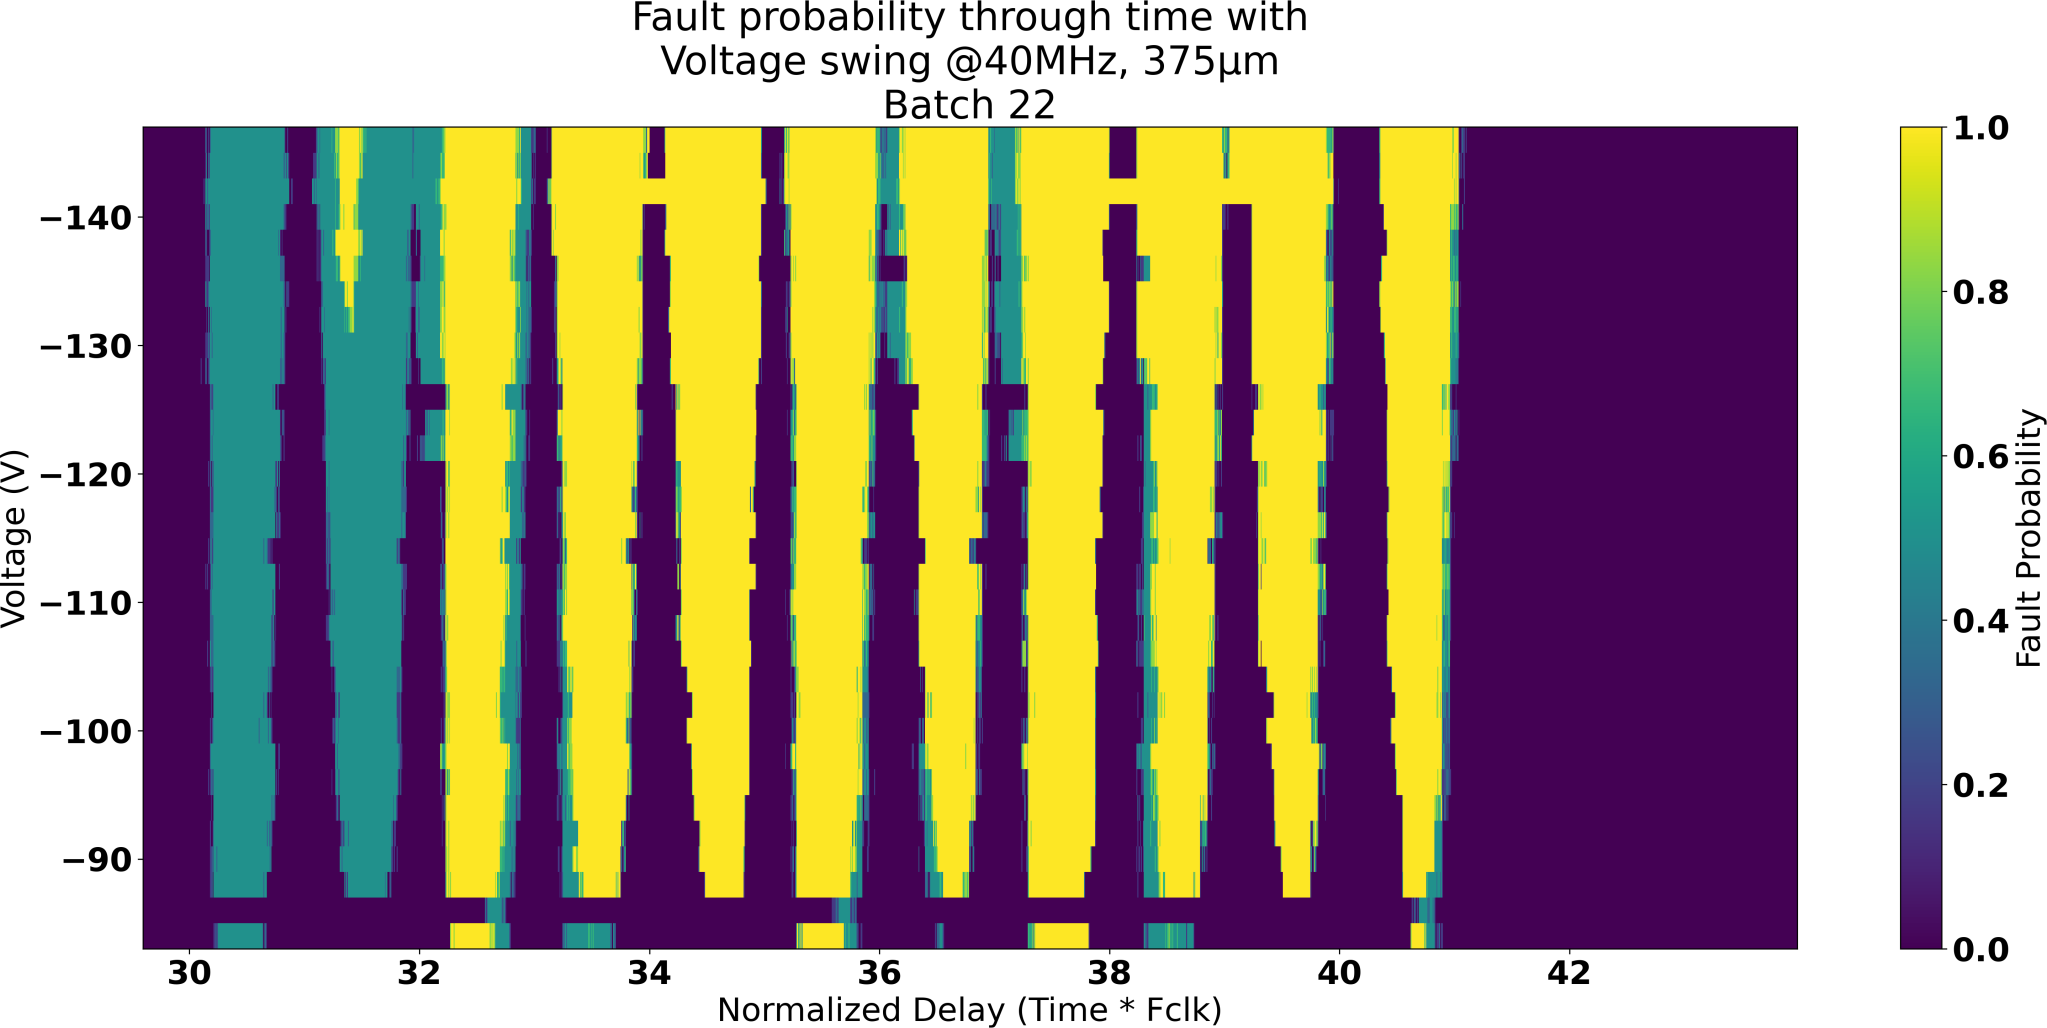
\includegraphics[width=\textwidth]{probafautes0.png}
            \end{textblock*}
            \begin{textblock*}{65mm}(20mm, 65mm)
                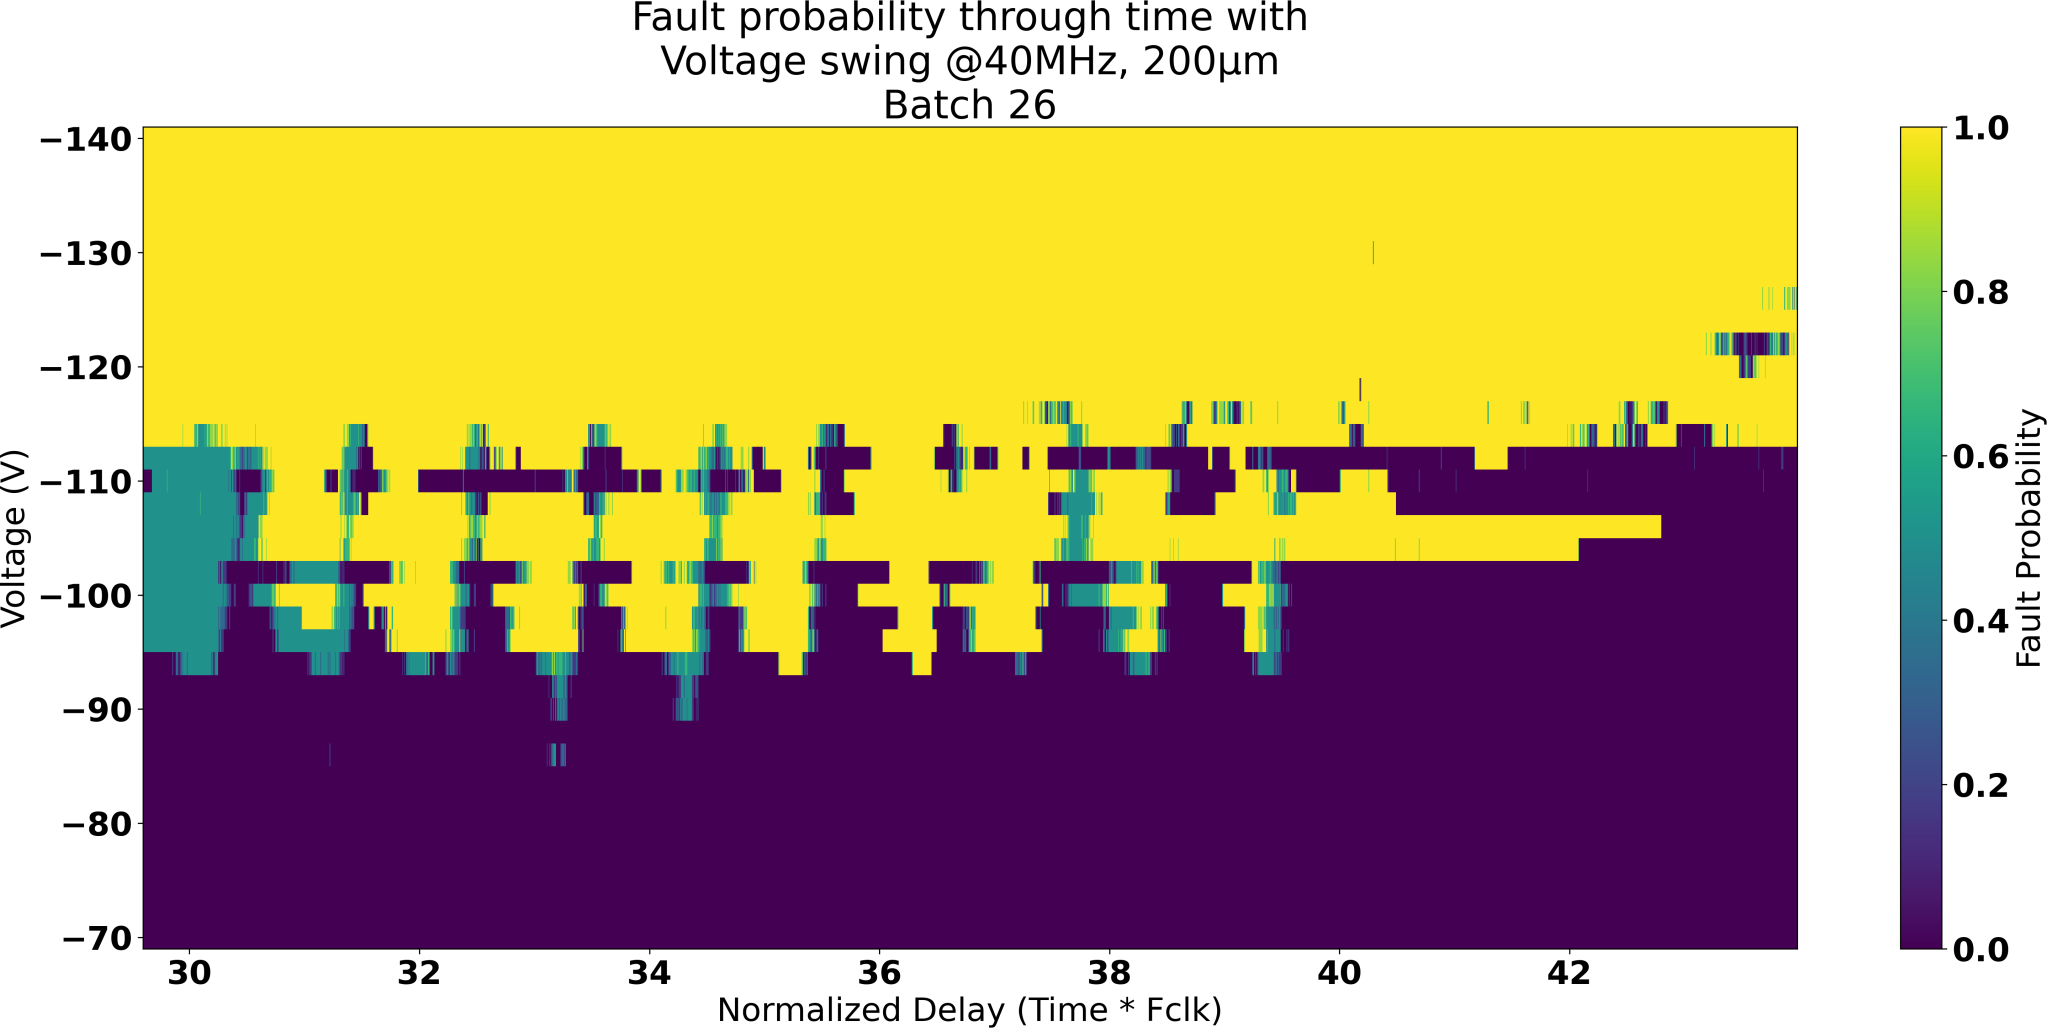
\includegraphics[width=\textwidth]{probafautes1.png}
            \end{textblock*}
        \end{column}
        %   Barre centrale
        \begin{textblock*}{1mm}(100mm, 20mm)
            
\begin{tikzpicture}
                \draw[-, black, line width=0.5mm] (0, 0) -- (0, 7.5);
            \end{tikzpicture}
        \end{textblock*}
        \begin{column}{0.33\textwidth}
            \centering
            \begin{figure}
                
\includegraphics[width=1.0\textwidth]{model0Probe.pdf}
            \end{figure}
            \vspace{-0.5cm}
            \begin{figure}
                \includegraphics[width=0.9\textwidth]{S1P.pdf}\\
                \includegraphics[width=0.9\textwidth]{S1G.pdf}
            \end{figure}
        \end{column}
    \end{columns}
\end{frame}
